\documentclass[12pt, twoside]{article}
\usepackage[francais]{babel}
\usepackage[T1]{fontenc}
\usepackage[latin1]{inputenc}
\usepackage[left=1cm, right=1cm, top=1cm, bottom=1cm]{geometry}
\usepackage{float}
\usepackage{graphicx}
\usepackage{array}
\usepackage{multirow}
\usepackage{amsmath,amssymb,mathrsfs}
\usepackage{soul}


\begin{document}


\section*{\center{Un th�or�me bien connu}}


\begin{tabular}{cc}
\begin{minipage}{14cm}
$ABC$ est un triangle recatngle en $A$ et $H$ le pied de la hauteur issue de
$A$.

\begin{enumerate}
  \item D�montrer que les triangles $ABC$, $ABH$ et $ACH$ sont semblables.
  \item Justifier que $AH^{2}=HB \times HC$, $AB^{2}=HB \times BC$ et
  $AC^{2}=BC \times HC$.
  \item En d�duire que $BC^{2}=AB^{2}+AC^{2}$. Enoncer le th�or�me d�montr�.
\end{enumerate}
\end{minipage}
&
\begin{minipage}{4cm}
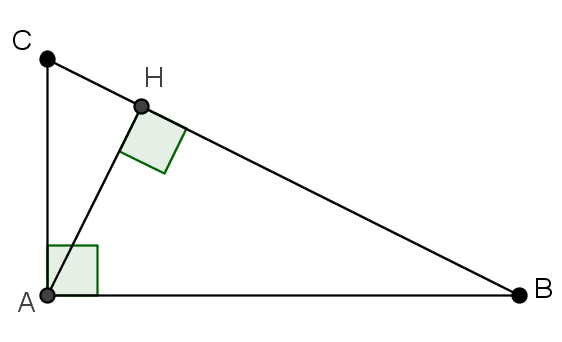
\includegraphics[width=4cm]{image/ex.png}
\end{minipage}
\end{tabular}

\section*{\center{Un th�or�me bien connu}}


\begin{tabular}{cc}
\begin{minipage}{14cm}
$ABC$ est un triangle recatngle en $A$ et $H$ le pied de la hauteur issue de
$A$.

\begin{enumerate}
  \item D�montrer que les triangles $ABC$, $ABH$ et $ACH$ sont semblables.
  \item Justifier que $AH^{2}=HB \times HC$, $AB^{2}=HB \times BC$ et
  $AC^{2}=BC \times HC$.
  \item En d�duire que $BC^{2}=AB^{2}+AC^{2}$. Enoncer le th�or�me d�montr�.
\end{enumerate}
\end{minipage}
&
\begin{minipage}{4cm}
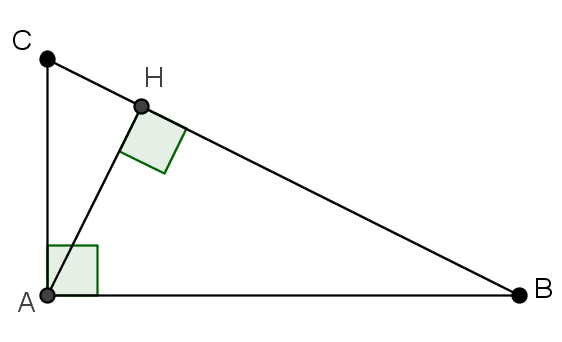
\includegraphics[width=4cm]{image/ex.png}
\end{minipage}
\end{tabular}

\section*{\center{Un th�or�me bien connu}}


\begin{tabular}{cc}
\begin{minipage}{14cm}
$ABC$ est un triangle recatngle en $A$ et $H$ le pied de la hauteur issue de
$A$.

\begin{enumerate}
  \item D�montrer que les triangles $ABC$, $ABH$ et $ACH$ sont semblables.
  \item Justifier que $AH^{2}=HB \times HC$, $AB^{2}=HB \times BC$ et
  $AC^{2}=BC \times HC$.
  \item En d�duire que $BC^{2}=AB^{2}+AC^{2}$. Enoncer le th�or�me d�montr�.
\end{enumerate}
\end{minipage}
&
\begin{minipage}{4cm}
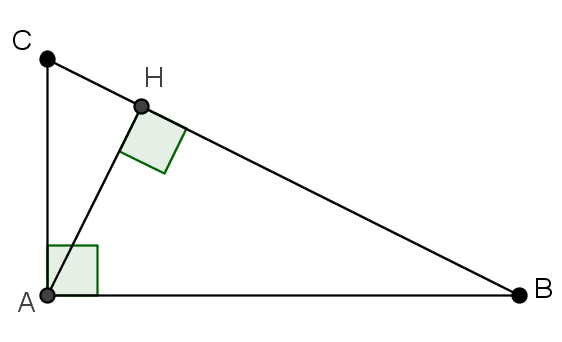
\includegraphics[width=4cm]{image/ex.png}
\end{minipage}
\end{tabular}

\section*{\center{Un th�or�me bien connu}}


\begin{tabular}{cc}
\begin{minipage}{14cm}
$ABC$ est un triangle recatngle en $A$ et $H$ le pied de la hauteur issue de
$A$.

\begin{enumerate}
  \item D�montrer que les triangles $ABC$, $ABH$ et $ACH$ sont semblables.
  \item Justifier que $AH^{2}=HB \times HC$, $AB^{2}=HB \times BC$ et
  $AC^{2}=BC \times HC$.
  \item En d�duire que $BC^{2}=AB^{2}+AC^{2}$. Enoncer le th�or�me d�montr�.
\end{enumerate}
\end{minipage}
&
\begin{minipage}{4cm}
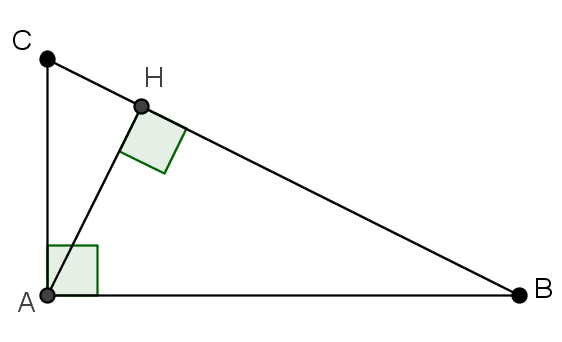
\includegraphics[width=4cm]{image/ex.png}
\end{minipage}
\end{tabular}

\section*{\center{Un th�or�me bien connu}}


\begin{tabular}{cc}
\begin{minipage}{14cm}
$ABC$ est un triangle recatngle en $A$ et $H$ le pied de la hauteur issue de
$A$.

\begin{enumerate}
  \item D�montrer que les triangles $ABC$, $ABH$ et $ACH$ sont semblables.
  \item Justifier que $AH^{2}=HB \times HC$, $AB^{2}=HB \times BC$ et
  $AC^{2}=BC \times HC$.
  \item En d�duire que $BC^{2}=AB^{2}+AC^{2}$. Enoncer le th�or�me d�montr�.
\end{enumerate}
\end{minipage}
&
\begin{minipage}{4cm}
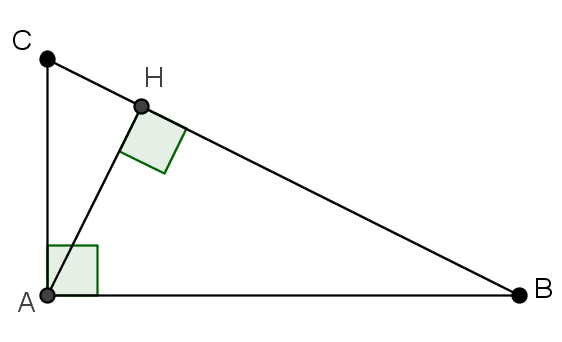
\includegraphics[width=4cm]{image/ex.png}
\end{minipage}
\end{tabular}

\end{document}
